%!TEX root = thesis.tex

\chapter{Simulator Plugin documentation}

\section{Implementation of the ROS control interface}

\subsection{Overview}

After finishing the modelling process it was necessary to find a proper way to control the robot components via a ROS control interface. The arm as well as the hand is controlled via a set of inbound and outbound ROS topics that allow to send commands to the underlying component or to receive state data from the component(joint states, sensor data,\ldots). Each simulated component should provide exactly the same interface as it's real counterpart.

One problem is how each type of component can be clearly identified within the current simulation scene. A scene is a hierarchy of various scene objects, organized in a tree structure. As already explained, those objects can be shapes, joints, sensors or even only dummies. The scene content can be modified by the user. Maybe a gripper gets replaced by another component, an arm gets removed or an additional Kinect camera gets installed. The required solution should be able to react to changes in the current scene. Parts of the model hierarchy should be clearly identifiable as a specific simulation component. Each single part of a component should be identifiable (joints, sensors, dummies, IK groups, collision objects). Luckily V-Rep provides various extension points for programmers and is therefore highly customizable. 

After some investigation about the possibilities the decision was made to create a simulator plugin, using the V-Rep regular API. This approach states the most flexible solution as this API provides more than 400 functions. A plugin is a compiled library file, written in C++ that has to follow some V-Rep specific naming conventions and must reside in the V-Rep working directory. The library file gets automatically loaded on V-Rep startup and runs in the main simulation thread. This means that it has to be programmed really carefully to avoid performance leaks during simulation. The plugin has to provide a clearly defined interface, consisting of 3 functions:

- v\_RepStart - called on startup and can handle some initialization
- v\_RepEnd - called before shutdown and can do some cleanup
- v\_RepMessage - called very often during the whole V-Rep lifecycle and is therefore a very
  performance critical method. Via this function V-Rep notifies the plugins about events like
  start/end of simulation, simulation step, scene content change, scene switch, \ldots.
  The plugin code can react to those events accordingly.


\subsection{Plugin Architecture}

\begin{figure}[ht]
	\centering
  	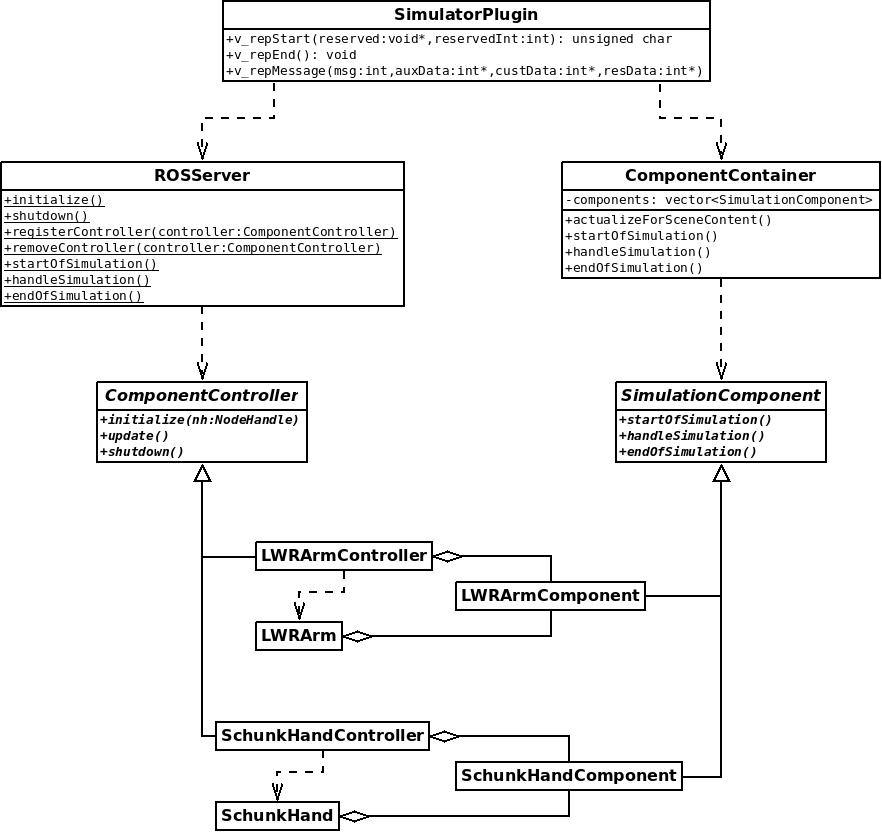
\includegraphics[width=1.0\textwidth]{images/SimulatorPluginUML.jpg}
	\caption{Simulator plugin architecture}
	\label{fig:plugin_uml}
\end{figure}
The plugin code is organized as can be seen in Figure\ref{fig:plugin_uml}.

- SimulationComponent
  A simulation component is a single, reusable part of the robot that can be used in different
  environments. Each component provides it's own clearly defined control interface. A simulation
  scene can contain various types of components. The SimulationComponent class is the abstract
  base class for all simulation components. Currently there are existing two concrete implementations
  -- the LWRArmComponent and the SchunkHandComponent. If the scenario should be extended and new
  components are introduced it is necessary to create a subclass of SimulationComponent and provide
  implementations for the abstract methods. Each SimulationComponent consists of two parts. The first 
  one is a class that provides access to a concrete simulation component instance. The LWRArm class
  for example stands for a KUKA LWR4+ arm model in the scene. This class provides full access to the
  functionality of the underlying arm model.
  
  The second part is a controller class for the component instance. This controller encapsulates the
  whole ROS interface to the simulation component and has to be a subclass of the abstract 
  ComponentController class. On each simulation pass the controller publishes all the necessary
  state data to it's various topics and sends incoming commands to the simulation component. The
  names of the various provided topics are composed from the overall namespace, the defined unique
  name of the component and the actual topic name. For example the joint control topic of the right
  robot arm evaluates to `/simulation/right\_arm/joint\_control/move'
  
  On simulation start each SimulationComponent registers it's ComponentController at the ROSServer
  and unregisters it on simulation end.
  
- ComponentContainer
  This class represents the set of all identified simulation components in the current simulation
  scene. On V-Rep startup an instance of ComponentContainer is created. Each time, the content of
  the current simulation scene changes, the method `ComponentContainer::actualizeForSceneContent' 
  is triggered. This method performs the following steps:
  - It validates each currently registered SimulationComponent instance if it is still valid and
    present in the scene.
  - It traverses the whole scene hierarchy to identify newly created components
  - If a new component is identified, a corresponding concrete instance of SimulationComponent 
    is created and added to the container.
  To identify a component it has to be marked by using V-Rep's custom developer data functionality.
  Details are explained further on.
  
  The ComponentContainer gets notified about each simulation step. It then simply forwards that
  message to all registered components. Those can then perform all necessary steps like triggering
  collision checking or the IK calculation module.
  
- ROSServer
  The ROSServer is a static class that encapsulates all ROS related functionality. It tries to 
  initialize ROS on startup. If the connection to the master can be established it creates a
  ROS NodeHandle for the `simulation' namespace. Otherwise it forces the plugin to unload, because
  it is not able to work without a running roscore.
  Each SimulationComponent registers it's ComponentController instance at the ROSServer. On 
  simulation start it initializes the registered controllers with the maintained NodeHandle. The
  ROSServer gets also notified about each simulation step and forces the controllers to handle the
  received commands and publish all the necessary data.
  On simulation end it forces the registered controllers to shutdown their publishers and 
  subscribers.
  
- ComponentController
  This is the abstract base class for all controllers. A ComponentController gets initialized by
  the ROSServer on simulation start. Concrete implementations can use the provided NodeHandle to
  create all the necessary publishers and subscribers. The update method is called by the ROSServer
  on each simulation step and forces the controller to publish all the required data. On simulation
  end the shutdown method is called by the ROSServer, forcing the controller to shutdown all 
  publishers and subscribers.
  
- LWRArm
  This class provides access to a correctly configured LWR arm model within the simulation scene.
  To fullfill the requirements for the control interface, the arm has to be able to operate in joint
  control mode and in inverse kinematics mode. Initially the arm starts in joint control mode. All 
  the joints are switched to torque/force mode and accept target positions to be set. The simulated
  PID controllers will try to move the joints to their designated target positions. 
  
  Switching to IK mode means to operate all the joints in IK mode and use the previously configured   
  IK calculation module. Setting a target pose in Cartesian space means to bring the IK target dummy
  into the required pose. The IK calculation module tries then to bring the linked IK tip dummy into
  the same pose by commanding the robot arm's joints accordingly and satisfying the configured
  constraints and precision settings. At the moment, three IK groups are configured for
  each arm with different settings to achieve performant and stable solutions. Those groups are
  sequentially called until one of them is successful. The configuration of the first group focuses
  on performance but provides less stability. The last group uses a configuration that is slower but
  provides more stability in positions closed to singularities. If none of the groups was successful
  it will result in an error message on the console, otherwise the arm will start or continue to move
  towards it's target pose. When initializing the LWRArmComponent, it will search for IK groups that 
  are named the same as the arm and with consecutive numbering (left\_arm, left\_arm1,
  left\_arm2,...).
  That allows to reconfigure the IK calculation module and introduce additional IK groups without 
  touching the plugin code. It is expected that at least one IK group is configured, otherwise
  an error message is written to the console.
  
  The collision status of the arm is determined by using the configured collision detection module.
  On each simulation step the collision group that is responsible for detecting direct collisions is 
  handled first. If that one detects a collision, a direct hit is reported and it is not necessary
  to handle the second group at all, because a direct hit always implies a hit with the shield as
  well. Only if no direct hit was detected, the second group is handled. The outcome can be queried
  as the current collision state of the arm. During initialization it is searched for a collision
  group that has the same name as the arm, responsible for direct hit detection and a group that is
  named with the naming pattern [arm\_nameShield], responsible for shield hit detection. If one or
  both of the required groups cannot be detected, an error message on the console will be stated and
  the collision detection functionality will not work as expected. Collision state is evaluated on 
  each simulation time step.
  
  Additional items that have to be identified within the model tree are the 7 joints, the end
  effector tip dummy, the IK target dummy and the force sensor on the last link of the arm. The
  origin of the reference frame can be defined by creating a dummy object within the scene with
  the special name 'ref\_frame\_origin'. If such a scene object is found, all Cartesian poses are
  taken with respect to the reference frame of that object, otherwise the poses are interpreted
  absolute within the world reference frame. All the necessary data that is published by the 
  controller can be accessed via this class.
  
- LWRArmController
  The LWRArmController provides the implementation of the Kukie interface. This interface is created
  by Simon Hangl especially for the KUKA arms in the IIS Lab.
  
\subsection{Identifying simulation components in the scene}
\begin{figure}[ht]
	\centering
  	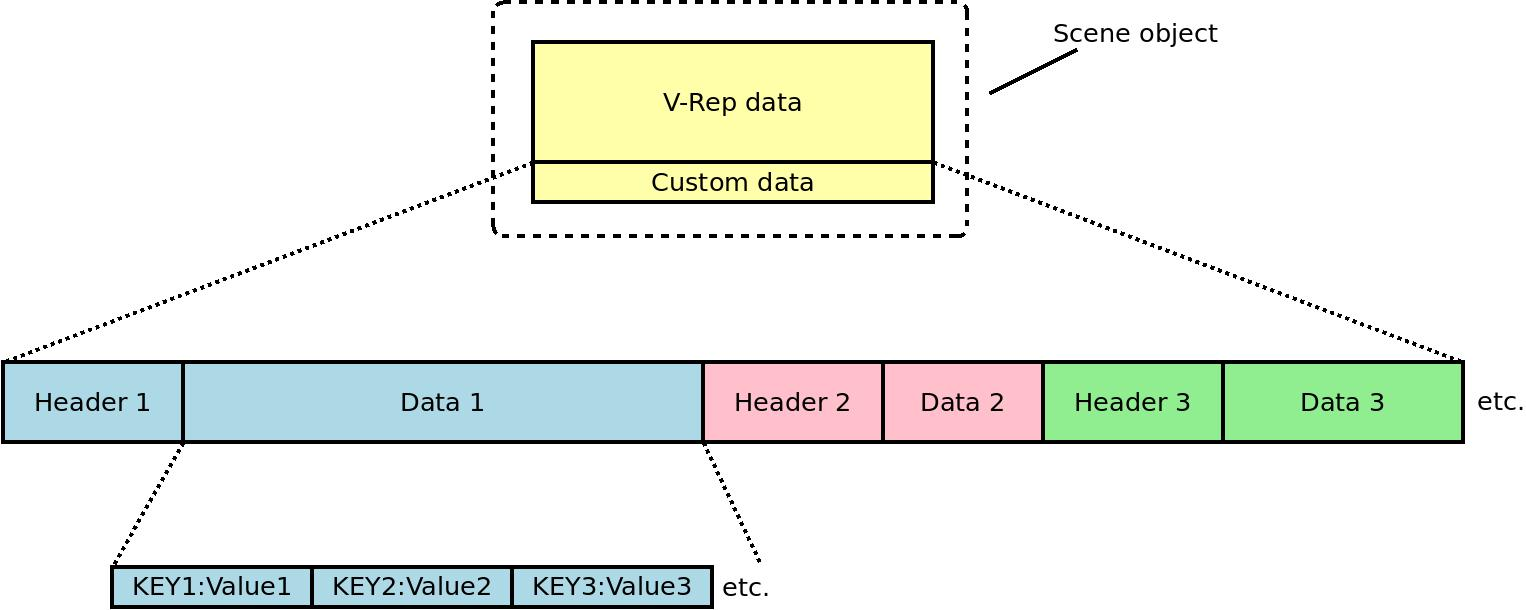
\includegraphics[width=1.0\textwidth]{images/custom_dev_data.jpg}
	\caption{Custom developer data segments on scene object}
	\label{fig:cust_dev_data}
\end{figure}
As each scene is a hierarchy of various types of scene objects there had to be found a way how to identify subtrees within this hierarchy that belong to known simulation components and should therefore be handeled by the plugin. One way would be to give each part a clearly defined, unique name and then search for those names within the scene. But than it would be necessary to hardcode the name of each single joint name and this is not a preferable solution for this problem. If somebody accidentally changes a name in the model tree then the solution is broken because the plugin looses connection to the underlying object and cannot control it any more. Here V-Rep's custom developer data functionality comes into play. It is possible to put auxiliary data segments to each single object in the scene.(TODO: show image of data segments) This data gets serialized together with the object and can be read programatically. Each data segment starts with a header number which is used to uniquely identify the data from a specific developer. The second element is an integer value that holds the length of the data segment and then comes the data itself. The format of the data can freely be chosen by the developer. It was decided to use string representations of key/value pairs, seperated by a colon (:). The key uniquely identifies the type of component (arm joint, hand joint, IK target dummy,...). The value segment can be used to provide additional data like for example the name of a joint. The left arm's model base for example is tagged with `2497,1:left\_arm'. This tag data item identifies that element as the model base of a LWRArmComponent with the name `left\_arm'. When actualizing for scene content change, the ComponentContainer traverses the scene hierarchy and looks for objects, that are tagged as known components. On success, it creates the specific instance with the object handle of the underlying scene object. During the initialization, the concrete SimulationComponent instance searches then the model subtree for all the necessary parts (joints, dummies, force sensors...). The implementations for the arm and the hand model provide feedback output on the console window about the success of this initialization process.

\subsection{Creating startup launch file}

Describe startup script, environmental variable (VREP\_PACKAGE\_PATH), launch file, how to use different simulation scenes.

\subsection{Documentation and usage examples}
Detailed documentation and implementation details should go into the Appendix


